\documentclass[12pt,fleqn]{article}\usepackage{../common}
\begin{document}
Ders 4

Bu derste diferansiyel denklemlerde ``degisken degistirme'' teknigini
gorecegiz. Onceki derslerde iki turlu ODE cozme yontemi
gorduk. Birinde degiskenleri ayirabiliyorduk, digeri lineer denklemler
idi. Isin ilginc tarafi o tur denklemler ve gosterilen cozumler her
zaman isleyen yegane ``genel'' yaklasimlardir. Digerler ODE'ler? Diger
tur denklemlerde degiskenin yerine bir baskasini gecirerek onu
kesinlikle cozebildigimiz bir forma indirgemeye ugrasiriz.

Ilk gorecegimiz degistirme teknigi olcekleme (scaling) olacak. 

Olcekleme, denklemin kullandigi kordinat sisteminde eksenleri (birini,
ya da hepsini) uzatip, kisaltmak anlamina gelir.

Diyelim ki $y' = f(x,y)$ formulumuz var. Yeni kordinat soyle olsun

\[ x_1 = \frac{x}{a} \]

\[ y_1 = \frac{y}{a} \]

$a,b$ sabit degerler. Boylece $x,y$ kordinatlarini olceklemis olduk.

Niye kordinat sistemini degistirmek isteriz? 1. Belki olcumlerin
birimini degistirmek istiyoruzdur (fizikte buna ihtiyac oluyor
mesela). 2. Bazen degiskenleri boyutsuz yapmak istiyor olabiliriz -kg,
cm birimler olmadan-, yani degistirdigimiz seyi hic bir birime sahip
olmayacak hale getirmek, sadece pur sayi yapmak. Fizikte birimlerle
bogusmanin dertleri malum. 3. Ya da ODE'deki sabit sayisini azaltmak
ya da sabitleri basitlestirmek icin bu yapilabilir.

Bir ornek gorelim. Bu ornek cok yuksek derecelerde kullanilan
soguma kanunudur. 

\[ \frac{dT}{dt} = k(M^4 - T^4) \]

T: ic sicaklik

M: sabit

Tekrarlayalim, bu kanun cok buyuk sicaklik farklarinda kullanilir,
cunku o seviyelerde Newton'un Soguma Kanunu islemiyor. 

Ilk degisimi yapalim, bu bir olcekleme operasyonu olsun. $T$ ve
$M$'nin arasinda bir baglanti kuralim. Yeni degisken $T_1$ olsun ve
soyle tanimlansin

\[ T_1 = \frac{T}{M} \]

$T$ degiskeni sicaklik belirttigi icin, celcius, fahrenheit gibi bir
birime sahipti, $M$ ayni sekilde. Ustteki bolumu yapinca sonuc
birimsiz bir hale gelecektir. Peki denklemdeki degiskeni nasil
degistirecegim? 

Yyerine gecirecegimiz degisken $T$ olduguna gore, o formda bir formul
kullanirsak daha iyi olur. Yani

\[ T = T_1M \]

ODE bu formule gore tekrar duzenlenirse

\[ M\frac{dT_1}{dt} = kM^4(1-T_1^4)\]

\[ \frac{dT_1}{dt} = k_1(1-T_1^4)  \]

$kM^3 = k_1$ dedik, yani yeni bir sabit yaratmis olduk, bu teknige
``sabitleri toparlama (lumping)'' adi veriliyor.

Ne degistirmis, ilerletmis olduk? Denklemin sag tarafi birimsiz hale
geldi ($T_1$ birimsiz). Sol tarafta tek birim zamanin tersi, yani
$zaman^{-1}$, $1/zaman$. Birimler azaldi. Ayrica artik denklemde bir
tane daha az sabit var, daha temiz duruyor.

Iki tur yerine gecirme (substitution) yontemi vardir. Biri direk
yontem, yeni bir degisken getirilir, bu degisken eskilerin bir tur
kombinasyonudur, onceki ornekte $T_1 = T / M$. Oteki tersine cevirme
(inverse), bu yontemde eski bir degisken eski ve yeni olanlarin bir
tur kombinasyonu olur, mesela $T = MT_1$. 

Bu farkliligi Calculus dersinde gormussunuzdur, hatirlatmak gerekirse,
tipik olarak su entegrali cozmek gerekince

\[ \int x \sqrt{1-x^2} dx \]

Yerine gecirmek icin $u = 1-x^2$ kullanilir, boylece $dx$ $du$ gecisi
yapilabilir, vs. Bu direk yontemin bir ornegi olurdu. Eger su olsaydi

\[ \int \sqrt{1-x^2} dx \]

ki $x = sin(u)$ kullanmak daha iyi olurdu. Bu da tersten yontemin bir ornegi.

Ornek

Direk Yerine Gecirme

\[ y' = p(x)y + q(x)y^n, \ \ \ \  n \neq 0,1 \]

Bu denkleme Bernoulli Denklemi denir. 

Denklemi $y^n$'e bolelim. 

\[ \frac{y'}{y^n} = p(x) \frac{1}{y^{n-1}} + q(x) \]

Bunu bir lineer denkleme cevirebiliriz, nasil? Yerine gecirme icin $v$
diye yeni bir degisken kurgulayalim:

\[ v = \frac{1}{y^{n-1}} = y^{1-n}\]

Turevi alalim

\[ v' = (1-n)\frac{1}{y^n}y' \]

Goruyoruz ki $v'$ ustte belirtilen $\frac{y'}{y^n}$ ile ayni (bir sabit
orani haric). O zaman denklemimizin yeni hali nedir?

\[ \frac{v'}{1-n} = p(x)v + q(x) \]

ki bu denklem lineer bir denklemdir. Hala standart formda degil ama o
degisimi hemen yapabiliriz. 

Ornek

\[ y' = \frac{y}{x} - y^2 \]

Bernoulli Denklemi 

\[ \frac{y'}{y^2} = \frac{1}{x}\frac{1}{y} - 1 \]

\[ v = \frac{1}{y}, v' = \frac{-1}{y^2}y' \]

\[ -v' = \frac{v}{x} - 1 \]

Standart form

\[ v' + \frac{v}{x} = 1 \]

Entegre edici faktor, $e^{ln(x)} = x$

\[ xv' + v = x \]

\[ (xv)' = x \]

\[ xv = \frac{1}{2}x^2 + C \]

\[ v = \frac{1}{2}x + \frac{c}{x} \]

Isimiz bitti mi? Hayir. Sonucu $y$ olarak almamiz lazim. 

\[ v = \frac{1}{2}x + \frac{c}{x} = \frac{x^2+2c}{2x}\]

$v = 1/y$ olduguna gore

\[ y = \frac{2x}{x^2+2c_1}\]

Tersine Cevirme Teknigi Ornegi

Homojen ODE

Homojen kelimesinin bir anlami ODE baglaminda esitligin saginda 0
oldugu durumdur, fakat simdi kullanilacak anlami degisik; buradaki
anlami su formdaki bir denklem demek

\[ y' = F(y/x) \]

Yani esitligin sag tarafinda ne zaman bir degisken gorursek, o
degiskenin $y/x$ ``turunde'' formunda oldugu turden bir denklem
(turunde derken ne demek istedigimizi birazdan anlatacagiz). Bazen bu
bolum form bariz olarak gozukmeyebilir, mesela

\[ y' = \frac{x^2y}{x^3 + y^3} \]

Fakat bu denklem homojendir, eger bolumun ustunu ve altini $x^3$'e
bolersek

\[ \frac{y/x}{1+(y/x)^3} \]

Goruldugu gibi bu denklem homojen. Peki su denklem?

\[ xy' = \sqrt{x^2 + y^2} \]

Bu da homojen. Iki tarafi da $x$'e bolelim, ve $x$'i $\sqrt{..}$ icine
tasirken onu $x^2$ yapmayi unutmayalim. Boylece

\[ y' = \sqrt{1+(y/x)^2} \]

Simdi turunde kelimesine gelelim: $y/x$ durumunun bir diger ifade
edilis tarzi sudur: Homojen ODE'ler buyutme, odaklanma (zoom)
operasyonu sonrasi degismezler (invariant under zoom). Yani sanki
kordinat sistemine zoom yaptigimizi, ufak bir noktayi buyuttugumuzu
farzedelim, eksen degisimi soyle,

\[ x = ax_1 \]

\[ y = ay_1 \]

Bu degisim sonrasi homojen denklemde hicbir degisiklik olmaz. 

Homojen ODE'leri nasil cozeriz?

\[ y' = F(y/x) \]

Degisken degistirme nasil yapariz? Soyle $z = y/x$. Fakat direk degil
tersten degistirme yontemini kullaniriz, direk kullansaydik $z'$
hesaplamak gerekecekti, fakat orada Bolum Kanunu vs. derken isler
sarpa saracakti. Daha basit olan tersten olan yontemi kullanmaktir. 
$y
= zx$. Niye boyle? Bu iyi bir kulaga kupe kuralidir: Aradigimiz sey
nedir? $y$'dir. O zaman $y$'yi degistirmeye ugrasmaliyiz.

\[ y = zx \]

\[ y' = z'x + z = F(z)\]

\[ x - \frac{dz}{dx} = F(z) - z \]

Goruyoruz ki degiskenler ayrilmis durumda. Entegral alarak gerisini
hallederiz. Tabii $z$'yi bulduktan sonra yerine koyarak $y$'ye
erismeyi unutmayalim. 

Problem

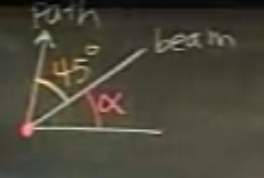
\includegraphics[height=2cm]{4_1.png}

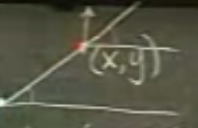
\includegraphics[height=2cm]{4_2.png}

Denizde bir isik kulesi (lighthouse) var, ve kuledeki kisi isigi
(beam) cevresinde istedigi yere yoneltebiliyor. Denizde bu isiga
yakalanmamak isteyen bir tekne var. Kule tekneye isigi yoneltince,
tekne ona 45 derece aciyla baska bir yere gitmeye calisiyor. Ardindan
kule hemen onu tekrar izliyor. Bu boyle devam ediyor. Soru: Geminin
takip edecegi yol (path) nedir? $x,y$ teknenin yerini temsil
etmektedir, $\alpha$, isigin x ekseni ile olan acisidir. 

\[ tan (\alpha) = \frac{y}{x} \]

\[ y' = tan(\alpha + 45) = \frac{tan(\alpha) + tan(45)}{1 - tan(\alpha)tan(45)} \]

\[ y' = \frac{y/x + 1}{1-y/x} =  \frac{y+x}{x-y} \]

Bolumun hem ustunu hem altini $x$ ile carpiyoruz, form daha guzel
gozukuyor. Ama ondan onceki formda, icinde $y/x$ olan form, zaten
denklemin homojen oldugunu belli ediyordu. 

\[ z = y/x \]

\[ y' = z'x + z \]

\[ z'x +z = \frac{z+1}{1-z} \]

Degiskenleri ayirmak istiyoruz, o zaman $z$'leri gruplayip bir tarafa
atalim. 

\[ x \frac{dz}{dx} = \frac{z+1}{1-z} - z = \frac{1+z^2}{1-z} \]

\[ \frac{1-z}{1+z^2}dz = \frac{dx}{x} \]

\[ \frac{1}{1+z^2} - \frac{z}{1+z^2} dz = \frac{dx}{x} \]


Iki tarafin entegralini alalim

\[ tan^{-1}z - \frac{1}{2} ln (1+z^2) = ln(x) + c \]

\[ tan^{-1}z = ln (1+z^2)^{1/2} + ln(x) + c \]

\[ tan^{-1}z = ln \sqrt{1+z^2} + ln(x) + c \]

\[ tan^{-1}(y/x) = ln (\sqrt{1+(y/x)^2}) + ln(x) + c \]

\[ tan^{-1}(y/x) = ln(x \sqrt{1+(y/x)^2}) + c \]

\[ tan^{-1}(y/x) = ln(\sqrt{x^2+y^2}) + c \]

Ustteki form kutupsal (polar) kordinatlarin formuna benziyor. Hakikaten:

\[ \theta = ln(r) + C \]

\[ r = C_1e^{\theta} \]

Ekler

Not: Kolay Sin ve Cos Hesabi

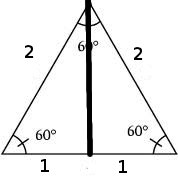
\includegraphics[height=2cm]{4_3.png}

45, 30, 60 gibi belli bazi acilar icin cabuk sin ve cos hesabi soyle
yapilabilir. 30 icin ustteki gibi esit kenarli ucgen dusunulur, bu ucgenin
ortasindan bir cizgi cekilir, ve ustte 30 derece, yani $\pi/6$, sagda 60
derece yani $\pi/3$ kalir. Cekilen cizginin boyu $\sqrt{2^2 - 1^2} =
\sqrt{3}$. Buna  gore $sin(30)$ nedir? Karsi bolu hipotenus = $1/2$. $cos(30)$ ayni ucgene 
gore $\sqrt{3}/2$ olur.

* * *

Alttakiler Ingilizce ders notlarindan aktariliyor:

Bir ``lineer ODE'', ``standart forma'' cevirilebilen bir denklemdir.

\[ r(t)x' + p(t)x = q(t) \]

$r(t)$ ve $p(t)$ katsayidir (coefficient). Denklemin sol tarafi ``sistemi''
temsil etmektedir, sag tarafi ise, bir anlamda, bir girdi (input) sinyalini
temsil etmektedir. Bu denklemin cozumu olan $x(t)$ ise sistemin cevabidir,
ya da cikti (output) sinyalidir. 

Bu denklemin tamamini $r(t)$'ye bolersek indirgenmis standart formu elde
ederiz. 

\[ x' + p(t)x = q(t) \]

Bu denklemin sag tarafindaki $q(t)$ eger sifir sinyali (null signal) ise,
yani $q(t) = 0$ degerindeyse, bu denkleme homojen denir. Bunun sezgisel
tercumesi sistemin izole bir halde evrildigi / degistigi / donustugu bir
durumdur: banka orneginde hic para yatirilmadigi, ve cekilmedigi, RC
(devre) orneginde ise devrede pil, enerji olmadigi, voltaj saglanmadigi bir
duruma tekabul eder. 

Homojen lineer denklem

\begin{equation}\label{4eq1}
x' + p(t) x = 0 
\end{equation}

ayirilabilir (seperable) bir denklemdir. Once ayir:

\[ dx/x = - p(t) dt \]

Entegre et

\[ ln|x| = - \int p(t) dt + c \]

Ustellestir (exponentiate)

\[ |x| = e^c e^{ - \int p(t) dt } \]

Mutlak (absolute) degeri elimine et ve kayip cozumu tekrar iceri sok

\[ x = C e^{- \int p(t) dt} \]

Eger $p(t) = 2t$ olsaydi ustteki basamaklar soyle olacakti

\[ x' + 2tx = 0 \]

\[ dx/x = - 2t dt \]

\[ ln|x| = - t^2 + c \]

\[ |x| = e^c e^{-t^2} \]

\[ x = C e^{-t^2} \]

Dikkat edin, ornekte $k$'nin belli bir anti-turevini kullandik, yani
$kt$. Bu entegralin ``gorulmeyen'' sabiti ilerideki basamaklarda ortaya
cikan $C$ tarafindan halledildi. 

Yani formul \ref{4eq1}'in genel cozumu $C x_h$ formundadir, ki $x_h$ sifir
olmayan herhangi bir cozumdur.

\[ x_h = e^{- \int p(t) dt} , \ x = C x_h \]

Ileride genel durumun bir cebirsel numara ile cozulebildigini ve iki
entegrasyon iceren bir dizi (sequence) ortaya cikardigini gorecegiz. 

Ekler

Icinde tanimsiz $C$ sabiti iceren cozum genel cozumdur, bu cozumler mumkun
olan ``tum cozum kumesini'' temsil ederler bir bakima. O sebeple
geneldirler. Ozel (particular) cozum baslangic sartlarini tatmin eden ve
$C$ icermeyen cozumlerdir. Entegral egrileri genel cozumun
grafikleridir. Her turlu $C$ olasiligi icin cizilmis egrilerdir onlar.

Bazen 

\[ x' + p(t)x = q(t) \]
 
formulunun tamami ayni anda tamamen cozulur ve $C$ iceren sonuc hemen elde
edilir. Ama bazen ustteki formule bagli olan homojen formulu cozmek daha
basit gelebiliyor, yani

\[ x' + p(t)x = 0 \]
 
cozuluyor, ve $x_h$ elde ediliyor. Sonra bir sekilde, belki tahmin ederek,
$x_p$ bulunuyor. Sonra su kurala siginilarak 

\[ x = x_p + cx_h \]

genel cozum o sekilde elde edilebiliyor. 

Ornek

\[ \dot{x} + tx = (1+t)e^t \]

Alakali homojen denklem 

\[ \dot{x} + tx = 0\]

Ayirilabilir bir denklem

\[ \frac{dx}{dt} + tx = 0 \]

\[ \frac{dx}{dt} = - tx  \]

\[ \frac{dx}{x} = -tx \]

\[ \int \frac{dx}{x} = \int -tx \]

\[ ln |x| = -t^2 / 2 + C \]

\[ x_h = e^{-t^2/2} \]

$C$ sabiti de var aslinda ama homojen cozum oldugu icin sabiti dahil
etmiyoruz, nasil olsa $x = x_p + cx_h$ tanimindan sabit dahil oluyor.

Simdi ozel cozumu $y_p$'yi nasil buluruz? Burada kullanilan tekniklerden
biri, $vx_h$, $v(t)$ yani $t$'nin bir fonksiyonu, seklinde cozumu homojen
cozumden ``uretebilecegimiz''. Bu ugrastigimiz turden lineer ODE'ler icin
hakikaten mumkun. $x_p$ bir sekilde bulunuyor demistik, iste sekillerden
biri bu. 

Teorisi:

$x=vx_h$ formulunu 

\[ x' + p(t)x = q(t) \]
 
yani standart forma sokuyoruz, 

\[ \dot{v}x_h + v\dot{x_h} + pvx_h = q \]

Ikinci ve ucuncu terim toplaninca sifir olur. Degil mi? Cunku $x_h$ homojen
denkleminin cozumu, o denklem de

\[ x' + p(t)x = 0 \]
 
seklinde. O zaman

\[ v\dot{x_h} + pvx_h = v(\dot{x_h} + px_h) = v \cdot 0 = 0 \]

Geriye kalan 

\[ \dot{v}x_h  = q \]

\[ \dot{v} = x_h^{-1} q \]

Direk entegrasyon ile $v$'yi buluruz, ozel cozumu temsil etmesi icin $v_p$
diyelim

\[ v_p = \int x_h^{-1} q dt\]

Yani 

\[ x_p = v_p x_h = x_h \int x_h^{-1} \ q \ dt \]

Ornegimize donersek

\[ x_h = e^{-t^2/2} \]
 
bulmustuk, o zaman 

\[ x_p =  e^{-t^2/2} \int e^{t^2/2} (1+t)e^t dt\]

Entegrali ayri olarak

\[ \int e^{t^2/2} (1+t)e^t dt  = 
\frac{e^{t+ t^2/2}}{(1+t)}{(1+t)} = 
e^{t+ t^2/2}
\]

\[ x_p =  e^{-t^2/2} e^{t+ t^2/2} \]

\[ x_p = e^t \]

Genel cozum 

\[ x = x_p + cx_h \]

\[ x = e^t + ce^{-t^2/2}  \]






\end{document}

